% This is "sig-alternate.tex" V2.1 April 2013
% This file should be compiled with V2.5 of "sig-alternate.cls" May 2012
%
% This example file demonstrates the use of the 'sig-alternate.cls'
% V2.5 LaTeX2e document class file. It is for those submitting
% articles to ACM Conference Proceedings WHO DO NOT WISH TO
% STRICTLY ADHERE TO THE SIGS (PUBS-BOARD-ENDORSED) STYLE.
% The 'sig-alternate.cls' file will produce a similar-looking,
% albeit, 'tighter' paper resulting in, invariably, fewer pages.
%
% ----------------------------------------------------------------------------------------------------------------
% This .tex file (and associated .cls V2.5) produces:
%       1) The Permission Statement
%       2) The Conference (location) Info information
%       3) The Copyright Line with ACM data
%       4) NO page numbers
%
% as against the acm_proc_article-sp.cls file which
% DOES NOT produce 1) thru' 3) above.
%
% Using 'sig-alternate.cls' you have control, however, from within
% the source .tex file, over both the CopyrightYear
% (defaulted to 200X) and the ACM Copyright Data
% (defaulted to X-XXXXX-XX-X/XX/XX).
% e.g.
% \CopyrightYear{2007} will cause 2007 to appear in the copyright line.
% \crdata{0-12345-67-8/90/12} will cause 0-12345-67-8/90/12 to appear in the copyright line.
%
% ---------------------------------------------------------------------------------------------------------------
% This .tex source is an example which *does* use
% the .bib file (from which the .bbl file % is produced).
% REMEMBER HOWEVER: After having produced the .bbl file,
% and prior to final submission, you *NEED* to 'insert'
% your .bbl file into your source .tex file so as to provide
% ONE 'self-contained' source file.
%
% ================= IF YOU HAVE QUESTIONS =======================
% Questions regarding the SIGS styles, SIGS policies and
% procedures, Conferences etc. should be sent to
% Adrienne Griscti (griscti@acm.org)
%
% Technical questions _only_ to
% Gerald Murray (murray@hq.acm.org)
% ===============================================================
%
% For tracking purposes - this is V2.0 - May 2012
\documentclass{sig-alternate-05-2015}

\usepackage{graphicx}
\usepackage{booktabs}
\usepackage[utf8]{inputenc}
\newcommand{\todo}{\textbf{TODO:} \textbf}

\begin{document}

% Copyright
%\setcopyright{acmcopyright}
%\setcopyright{acmlicensed}
%\setcopyright{rightsretained}
%\setcopyright{usgov}
%\setcopyright{usgovmixed}
%\setcopyright{cagov}
%\setcopyright{cagovmixed}
% DOI
%\doi{10.475/123_4}
% ISBN
%\isbn{123-4567-24-567/08/06}
%Conference
%\conferenceinfo{PLDI '13}{June 16--19, 2013, Seattle, WA, USA}
%s\acmPrice{\$15.00}
%
% --- Author Metadata here ---
%\conferenceinfo{WOODSTOCK}{'97 El Paso, Texas USA}
%\CopyrightYear{2007} % Allows default copyright year (20XX) to be over-ridden - IF NEED BE.
%\crdata{0-12345-67-8/90/01}  % Allows default copyright data (0-89791-88-6/97/05) to be over-ridden - IF NEED BE.
% --- End of Author Metadata ---
\title{Analysis of the efficiency and user satisfaction of a menu and swipe gestures in the context of a survey app}
%
% You need the command \numberofauthors to handle the 'placement
% and alignment' of the authors beneath the title.
%
% For aesthetic reasons, we recommend 'three authors at a time'
% i.e. three 'name/affiliation blocks' be placed beneath the title.
%
% NOTE: You are NOT restricted in how many 'rows' of
% "name/affiliations" may appear. We just ask that you restrict
% the number of 'columns' to three.
%
% Because of the available 'opening page real-estate'
% we ask you to refrain from putting more than six authors
% (two rows with three columns) beneath the article title.
% More than six makes the first-page appear very cluttered indeed.
%
% Use the \alignauthor commands to handle the names
% and affiliations for an 'aesthetic maximum' of six authors.
% Add names, affiliations, addresses for
% the seventh etc. author(s) as the argument for the
% \additionalauthors command.
% These 'additional authors' will be output/set for you
% without further effort on your part as the last section in
% the body of your article BEFORE References or any Appendices.
\numberofauthors{4} %  in this sample file, there are a *total*
% of EIGHT authors. SIX appear on the 'first-page' (for formatting
% reasons) and the remaining two appear in the \additionalauthors section.
\author{
  % You can go ahead and credit any number of authors here,
  % e.g. one 'row of three' or two rows (consisting of one row of three
  % and a second row of one, two or three).
  %
  % The command \alignauthor (no curly braces needed) should
  % precede each author name, affiliation/snail-mail address and
  % e-mail address. Additionally, tag each line of
  % affiliation/address with \affaddr, and tag the
  % e-mail address with \email.
  %
  % 1st. author
  \alignauthor
  Lukas Galke\\
  \affaddr{Kiel University, Germany}\\
  \email{lga@informatik.uni-kiel.de}
  % 2nd. author
  \alignauthor Steffen Goos\\
  \email{stg@informatik.uni-kiel.de}
  \and  % use '\and' if you need 'another row' of author names
  % 3rd. author
  \alignauthor
  Felix Paur\\
  \email{mail@uni-kiel.de}
  % 4th. author
  \alignauthor
  Florian Mai\\
  \email{mail@uni-kiel.de}
}
% There's nothing stopping you putting the seventh, eighth, etc.
% author on the opening page (as the 'third row') but we ask,
% for aesthetic reasons that you place these 'additional authors'
% in the \additional authors block, viz.
%\additionalauthors{Additional authors: John Smith (The Th{\o}rv{\"a}ld Group,
%email: {\texttt{jsmith@affiliation.org}}) and Julius P.~Kumquat
%(The Kumquat Consortium, email: {\texttt{jpkumquat@consortium.net}}).}
%\date{30 July 1999}
% Just remember to make sure that the TOTAL number of authors
% is the number that will appear on the first page PLUS the
% number that will appear in the \additionalauthors section.
\maketitle
% Fakesection ACM Header
\begin{abstract}
  For several years, the swipe gesture has been a very-well established way to navigate among adjacent pages on websites as well as in native
  apps on a mobile device. The users appreciate its ease and its comfort of use. However, it can only be applied in scenarios where
  the content is provided in a sequential way, e.g.\ in a picture gallery, in an e-book reader, or when filling in a form. In this paper, we
  examine the swipe gesture's suitability for navigating through a set of questions in an e-learning app. Although typically the user progresses
  through the questions sequentially, it is a common case that they want to revise their answers later due to a change of mind or a missunderstanding
  of the question, for example. We conjecture that navigating back using swipe gestures is unsatisfactory and time-costly as the distance in pages
  increases. In order to research this question, we conduct a study in which we compare the use of swipe gestures to the use of the also
  well-established hamburger menu. We design tasks that capture the use cases described above. We alter the distance in pages
  that has to be covered in order to complete the task. For each task, we measure the efficiency. Furthermore, we assess the user satisfaction through a questionnaire. We expect
  both measures to be independent of the distance when the menu is used. When the swipe gesture is used, however, we expect both measures to decrease
  as the distance increases. We suspect that the swipe gestures do better than the menu when the distance is small, but we also think that this relation flips at a number of pages that is realistic for e-learning apps. Hence, the results of our study are of practical importance.
\end{abstract}
%
% The code below should be generated by the tool at
% http://dl.acm.org/ccs.cfm
% Please copy and paste the code instead of the example below.
%
\begin{CCSXML}
  <ccs2012>
  <concept>
  <concept_id>10010520.10010553.10010562</concept_id>
  <concept_desc>Computer systems organization~Embedded systems</concept_desc>
  <concept_significance>500</concept_significance>
  </concept>
  <concept>
  <concept_id>10010520.10010575.10010755</concept_id>
  <concept_desc>Computer systems organization~Redundancy</concept_desc>
  <concept_significance>300</concept_significance>
  </concept>
  <concept>
  <concept_id>10010520.10010553.10010554</concept_id>
  <concept_desc>Computer systems organization~Robotics</concept_desc>
  <concept_significance>100</concept_significance>
  </concept>
  <concept>
  <concept_id>10003033.10003083.10003095</concept_id>
  <concept_desc>Networks~Network reliability</concept_desc>
  <concept_significance>100</concept_significance>
  </concept>
  </ccs2012>
\end{CCSXML}
\ccsdesc[500]{Computer systems organization~Embedded systems}
\ccsdesc[300]{Computer systems organization~Redundancy}
\ccsdesc{Computer systems organization~Robotics}
\ccsdesc[100]{Networks~Network reliability}
%
% End generated code
%
%
%  Use this command to print the description
%
\printccsdesc
% We no longer use \terms command
%\terms{Theory}
\keywords{mobile application, swipe, hamburger menu, learning application}


\section{Introduction}
Due to the availability of mobile internet connection and the establishment of
smartphones for the masses, e-learning applications have become more and more relevant in recent years.  In theory, the promise is that students can study anywhere at any time. However, as for any kind of application, a practical barrier is the usability of such educational application.
\begin{figure}[h]
	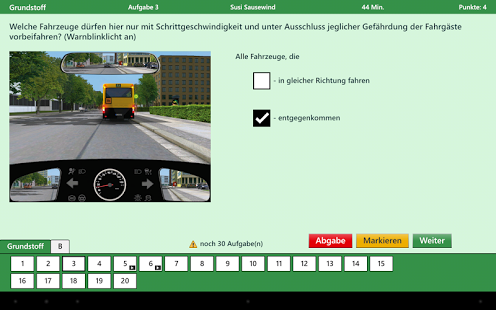
\includegraphics[width=\columnwidth]{drivinglicense.png}
	\caption{Mobile application 'Fahren Lernen Max'}
	\label{fig:fahren_lernen}
\end{figure}
For several years, the swipe gesture has been a very well-established way to
navigate among adjacent pages on websites as well as in native applications on a mobile device (Apps). The users appreciate its ease and comfort of use. However,
it can only be applied in scenarios where the content is provided in a
sequential way, e.g.\ in a picture gallery, in an e-book reader, or when
filling in a form. In this paper, we examine the swipe gesture's suitability
for navigating through a set of questions in an e-learning apps.
\begin{figure*}[!h]
	\centering
	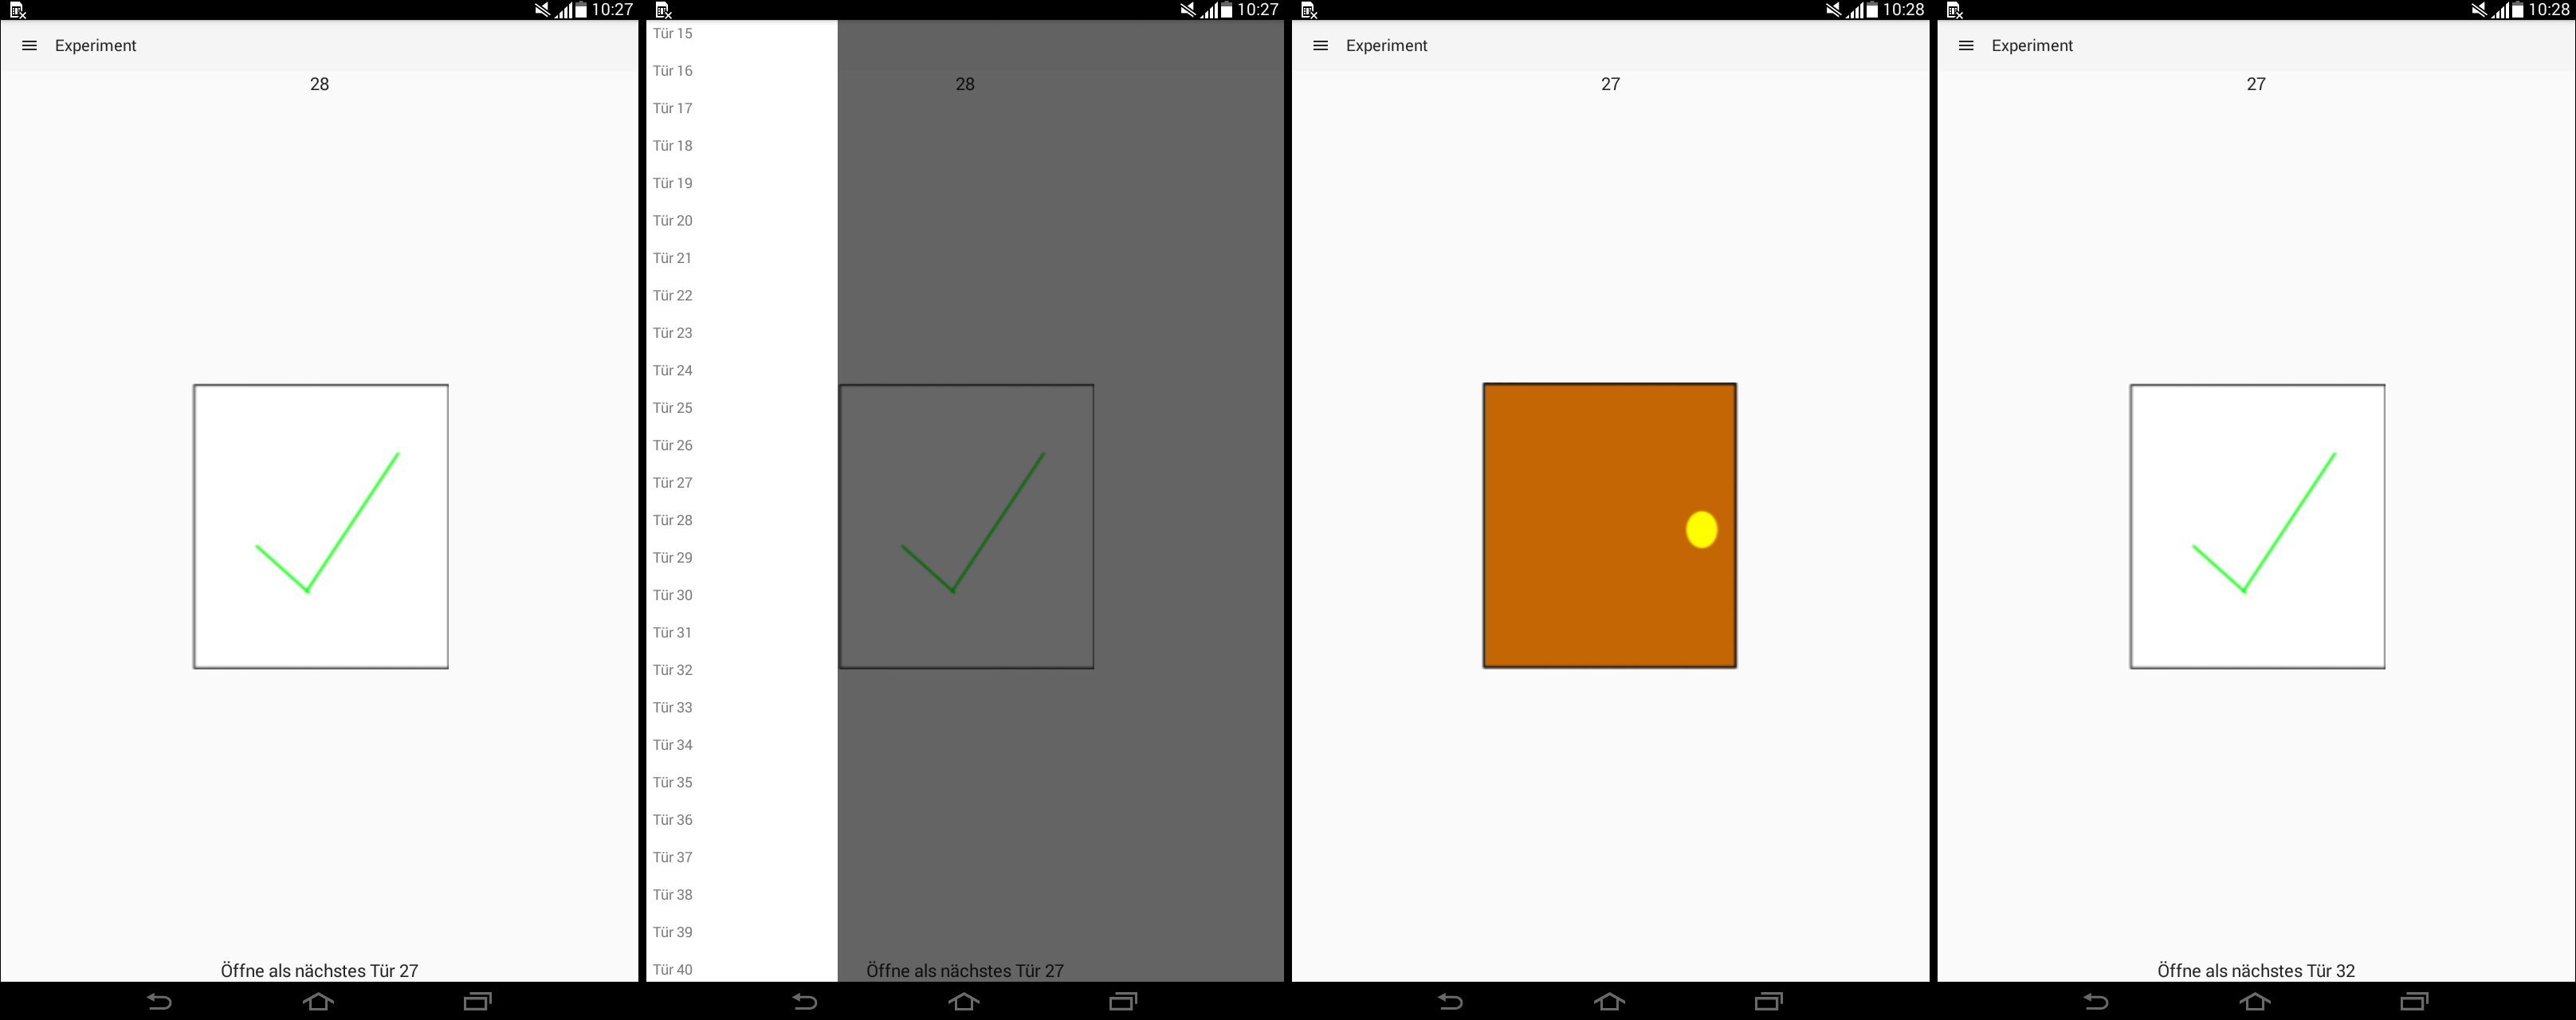
\includegraphics[width=\linewidth]{pics/screenshots/sequence}
	\caption{Hamburger navigation sequence}
	\label{fig:sequence}
\end{figure*}
Although typically the user progresses through the questions sequentially, it is a
common case that they want to revise their answers later due to a change of
mind or a misunderstanding of the question, for example. A case that applies very
well to this scenario is the theory test that has to be passed in order to obtain
a driving license in Germany. It consists of a relatively large number of questions and it's common practice to prepare for this examination by taking several exemplary tests. For example, consider Figure \ref{fig:fahren_lernen} which displays a screenshot of the
mobile application 'Fahren Lernen Max'. It displays the typical environment that
is also used for the actual exam. Questions are ordered sequentially, but the examinees
may answer them in any order. During examinations, it is common that some questions are
skipped and returned to at some later point.

In the example of this application, navigation between questions can be done via menu at the bottom of the screen in any direction or via button 'Weiter' only forward. Our goal is to find a generalizable statement about what navigation methods makes sense in these scenarios. We conjecture that navigating backward using swipe gestures is unsatisfactory and time-costly as the distance in pages increases. In order to research this question, we conduct a study in which we compare the use of swipe gestures to the use of the also well-established hamburger menu. This kind of navigation is mostly represent by three horizontally lines on the left or right upper corner of the screen. By touching the hamburger button a menu appears at the side of the screen. We suspect that the swipe gestures do better in terms of efficiency and user satisfaction than the hamburger menu on small distances. However, if the distance is large we believe that this relation flips.


\section{Apparatus}
In order to simulate the scenarios of jumping from one question to another, we develop a series of treasure hunt like tasks. Here, the goal is to find the treasure which is hidden behind a door. A door is represented by a page. The application was developed for Android devices. We have used two Samsung Galaxy Note 10.1 with Android 4.4.2 for our data collection.

First of all an initial page containing the identification number of the participant is shown so the task can be linked to the demographic questionnaire at the very end. Starting at the first page, an instruction displayed on the bottom of the screen guides the participant to the next one by exactly telling them the number of the next door. Now the participant has the possibility to navigate to the next door by swiping left or right, or using the hamburger menu (Figure \ref{fig:sequence}) on the upper left corner. The navigation method depends on the group in which they are located. When the participant has open the respective door, the next instruction is displayed. The distance $d$ to cover from one door to another is always about the same ($d \pm 1$\textit{, see Section \ref{sec:task}}) within the same task. However, the distances differ for different tasks. Consider the example in Figure \ref{fig:jump} which has distance of two. The arrows indicate the door to open in the next step and the arrow captions show the jump distance. Hence, the sequence of doors to open in order to reach the treasure is 2, 4, 1, 3, 5, 6.
\begin{figure}
	\centering
	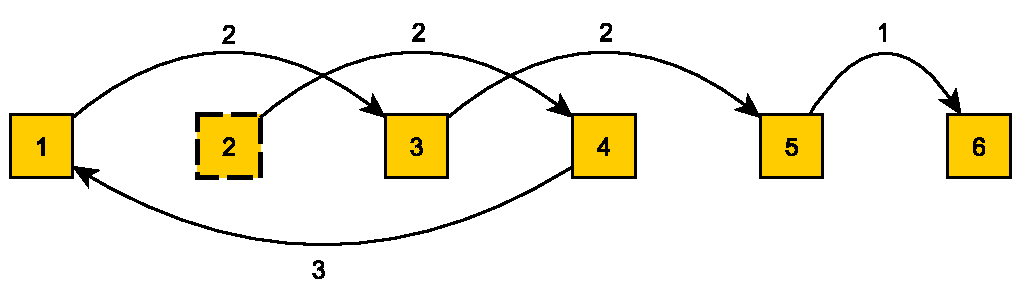
\includegraphics[width=0.45\textwidth]{pics/jump}
	\label{fig:jump}
	\caption{Example of a distance-two-jump}
\end{figure}
\begin{figure}
	\centering
	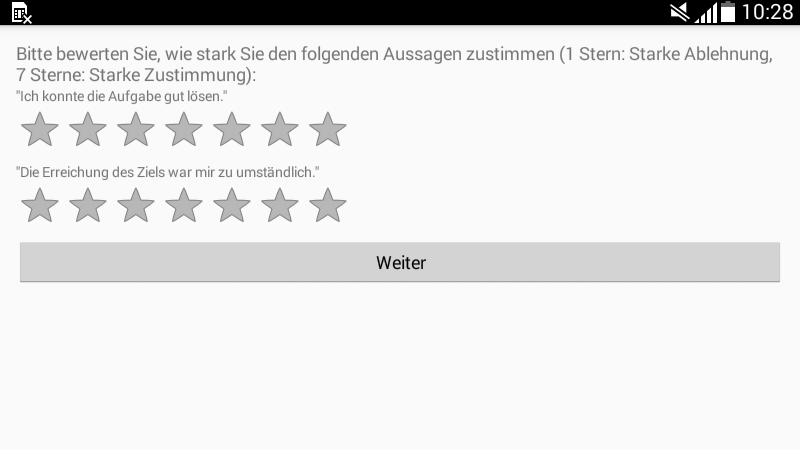
\includegraphics[width=0.475\textwidth]{pics/screenshots/global3-cut}
	\label{fig:between_questionnaire}
	\caption{Between questionnaire}
\end{figure}
The tasks cannot be failed to be completed because there is no way to open the doors in the wrong order. The participant has to complete a training set and five task sets. Every set consists of five jumping instructions. After each set the participant has to answer two questions (see Section \ref{sec:measurements}) and at the very end there will be a questionnaire of four questions.
\begin{figure}
	\centering
	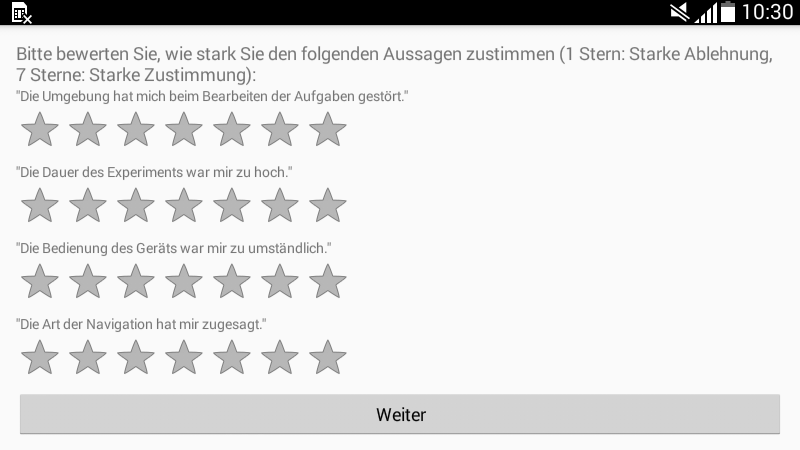
\includegraphics[width=0.475\textwidth]{pics/screenshots/global5-cut}
	\label{fig:final_questionnaire}
	\caption{Final questionnaire}
\end{figure}
\section{Evaluation Design}
\subsection{Procedure}
For our study, we decided for a between-group design for two reasons. First,
when solving the tasks with the second type, the test persons might rate their
satisfaction more drastically, as they are biased from having solved the tasks
with the respective other navigation method. Secondly, in order to avoid an
extreme learning effect, the tasks for swipe gesture navigation and menu
navigation would have to be distinct if a within-group design were used. This
should be avoided to ensure comparability. The participants are assigned to
each group randomly (at uniform) by employing the random number generator of
the respective android device.

The entire flow for one participant is as follows: First, the participant is explained
the purpose of the study (evaluation of navigation methods on mobile (touch)-devices) and the
type of task to solve (navigation through app). After completing an informed consent form, a unique
identifier is generated and handed over to the participant alongside contact information. Since often students
stay in the dining hall in groups, the participant is separated from the group in order to avoid distraction. 
Before the actual experiment starts, the participant completes a training task during which the goal, the
different layout items, and the navigation are explained. Before finishing the questionnaire for the training
task, the participant is informed that the experiment will start and is asked to focus on the tasks. When they have
finished, the last step for them is to provide demographical data age, gender, profession (including field of study),
and whether they own a smartphone with an Android operating system, a different operating system, or no smartphone.

\subsection{Participants}
Since our target scenario is an application used during examinations,
a typical user of such an application is a university student. Hence, the participants were acquisited in a field study conducted in an academic context, namely the dining hall of Christian-Albrechts-University in Kiel. The participants are representative for all students as the statistics show: In total, there are $N = 50$ participants. All of them are students and the most common courses are: economic computer science (12 \%), agricultural sciences (10 \%), mathematics (8 \%), psychology (8 \%) and economics (6 \%). For the entire distribution consider table \ref{tab:course}. The participants split up into 42 \% male and 58 \% female. The average age is 24.1 (SD: 2.9), 
with values between 20 and 35. 
All but one of the participants own a
smartphone, 75.51 \% of which run Android. This indicates that we may assume good knowledge
of how to handle the device used in our experiment.
The participants signed an informed consent form before the start of the experiment. After
finishing the experiment, they were rewarded with sweets or fruits.

\subsection{Tasks}
\label{sec:task}
During task creation, we faced several design issues: In order to avoid learning effects and for the results to generalize better, 
the sequence should require both forward- and backward-jumps. This raises the problem of collisions, that is, a door is visited twice, which
should also be avoided due to a learning effect. Hence, it is not possible to always have the exact same distance from one door to the
next in the sequence without collisions, but instead they have to differ slighly. However, it is always possible to create a non-colliding sequence of
length five by using distances $d$ three times and distances $d - 1$ and $d + 1$ once each. Hence, on average we have a distance of $d$. 
Furthermore, the distances being limited to two neighbored values, it is reasonable to assume negligible
impact on the experiments outcomes in terms of user-satisfaction and time.

To further reduce any bias of learning effects
the concrete permutation of tasks is generated by subsequently drawing
(uniformly at random, without returning) from the remaining tasks.

For the concrete tasks, please see the appendix. 
\todo{All tasks should always have the same number of doors (although the jump distances remain different)}
\subsection{Measurements}\label{chap:measurements}
\label{sec:measurements}
As stated above, we aim to measure the common three dependent variables efficiency, satisfaction, and effectiveness of each of the two navigation methods.
\paragraph{Effectiveness}
During the experiment, the application tracks how often the page is changed by the user, that is by either swiping or selecting a different page in the menu. 
Given some task that requires 5 jumps, where the distances to cover in the jumps are given as $d_i, 1 \leq i \leq 5$, let $n_{interactions_i}$ be the number
of page changes by the user for jump $i$.
The optimal number $n_{opt_i}$ of
page changes required equals $1$ for the burger menu navigation and $d_1$ for the swipe gesture navigation. As a measure of 
effectiveness, we measure in how many of the jumps unnecessary page changes were made, that is, the effectiveness for a task
equals $\frac{|\{i \in \{1,\ldots,5\} | n_{interactions_i} = n_{opt_i} \}|}{5}$.
\paragraph{Efficiency} For the efficiency, we calculate the effectiveness of a task required divided by the time 
required to complete the task in milliseconds. We start measuring the time at the point
when the first instruction is displayed and stop when the last door is opened.
\paragraph{Satisfaction}
In order to assess the user satisfaction depending on the distance, after each task, the user is asked to estimate their
agreement on two statements concerning the task. The statements are the following.
\begin{enumerate}
  \item 'I was able to solve the task well.' (in German: 'Ich konnte die Aufgabe gut loesen.')
  \item 'Achieving the goal was too intricate.' (in German: 'Die Erreichung des Ziels war mir zu umstaendlich.')
\end{enumerate}
The rating scale follows the common 7-likert-scale from strongly disagree (1) to strongly agree (7). \todo{Need to justify why 7?}
The first statement will be used to quantify whether the participants have understood the task and how to solve it. The second statement will
be used to quantify the participant's satisfaction with the navigation method.
After all tasks were completed, the participant also rates these statements that aim to assess the overall experience throughout the experiment.
\begin{enumerate}
  \item 'The environment during working on the tasks was disturbing.' (German: 'Die Umgebung hat mich beim Bearbeiten der Aufgaben gestoert.')
  \item 'The duration of the experiment was too high.' (German: 'Die Dauer des Experiments war mir zu hoch.')
  \item 'Handling the device was intricate.' (German: 'Die Bedienung des Geraets war mir zu umstaendlich.')
  \item 'The type of navigation was appealing to me.' (German: 'Die Art der Navigation hat mir zugesagt.')
\end{enumerate}
Question (1) and (2) serve the purposes to check whether the quality the experiment's results is impaired due to the lack of a laboratory environment or
due to participants' fatigue, respectively. \todo{What is question (3) good for?} Question (4) directly assesses the overall satisfaction with the navigation method.
\todo{Why is final question (4) different to task question (2)?}
\section{Evaluation Results}
%%%%%%%%%%%%%%%%%%%%%%%%%%%%%%%%%%%%


More formally: Let $d$ be the distance in pages to be covered when navigating in a sequence of pages. We formulate the following hypotheses:
\begin{enumerate}
	\item Null hypothesis $H_0^{(e)}$ for efficiency:
	There is no difference between swipe gestures and hamburger menu in the
	time required to navigate over a distance of $d$ pages.
	\item Alternative hypothesis $H_1^{(e)}$ for efficiency: There is a
	difference between swipe gestures and hamburger menu in the time required
	to navigate over a distance of $d$ pages.
	\item Null hypothesis $H_0^{(s)}$ for user satisfaction: There is no
	difference in user satisfaction between swipe gestures and hamburger menu
	when navigating over a distance of $d$ pages.
	\item Alternative hypothesis $H_1^{(s)}$ for user satisfaction: There is a
	difference in user satisfaction between swipe gestures and hamburger menu
	when navigating over a distance of $d$ pages.
\end{enumerate}

\paragraph{Hypotheses}
\todo{begin: MERGE WITH ABOVE}
Consider the normally distributed random variables $X_d$ with means $\bar x$ and
variances $\sigma_x^2$ being the time required for traveling $d$ pages using Hamburger
Menu navigation.
We hypothize that
\begin{align*}
	H_{0, \text{burger}}: \bar x_0 = \bar x_1 = \cdots = \bar x_d
\end{align*}
% is anova capable of doing reverse test with \not= as H_0?
Since we can assume equal variances,
we evaluate the hypothesis using {ANOVA}.
In case we do not find significant differences, we can use the overall mean
$\bar x$ for comparision with the Swipe navigation. 
We consider normally
distributed random variables $Y_d$ with means $\bar y_d$ and variances $\sigma_{y,d}^2$ as the
time required for traveling $d$ pages using Swipe navigation. 
After asserting
that analogous hypothesis for Swipe navigation fails,
\begin{align*}
	H_{0, \text{swipe}}: \bar y_0 = \bar y_1= \cdots = \bar y_d
\end{align*}
we continue with comparing the means $\bar y_d$ of Swipe navigation to the
mean $\bar x$ of Hamburger Menu navigation.  In order to find the distance
$d$, for which the required time with Swipe navigation exceeds the required
time with Hamburger Menu navigation, we formulate the following hypotheses:
\begin{align*}
	H_{0,d} : \bar y_d = \bar x \;\forall d
\end{align*}
\todo{end, reread.\ this might be moved to a later section, since it is
	quite technical already}


In fact, we check these hypotheses for different values of $d$, hence, we
examine two independent variables: navigation method and distance. We talked to
experts from the educational science domain to identify values for $d$ that
are realistic for e-learning apps. The talk revealed that a typical block
contains no more than $25$ questions. We are confident to be able to show statistical
superiority of swipe gestures for small $d$ and the superiority of hamburger
menu for large $d$ statistically for both quantities.  To be more precise, we
expect the relation between $d$ and the time required to navigate between
pages of distance $d$ as indicated in Figure~\ref{fig:expectation}.
\begin{figure}
	\caption{Expected time (y-axis) required to cover $d$ pages (x-axis) when using a menu (green line) and when using swipe gestures (blue line)}
	\resizebox{\columnwidth}{!}{
		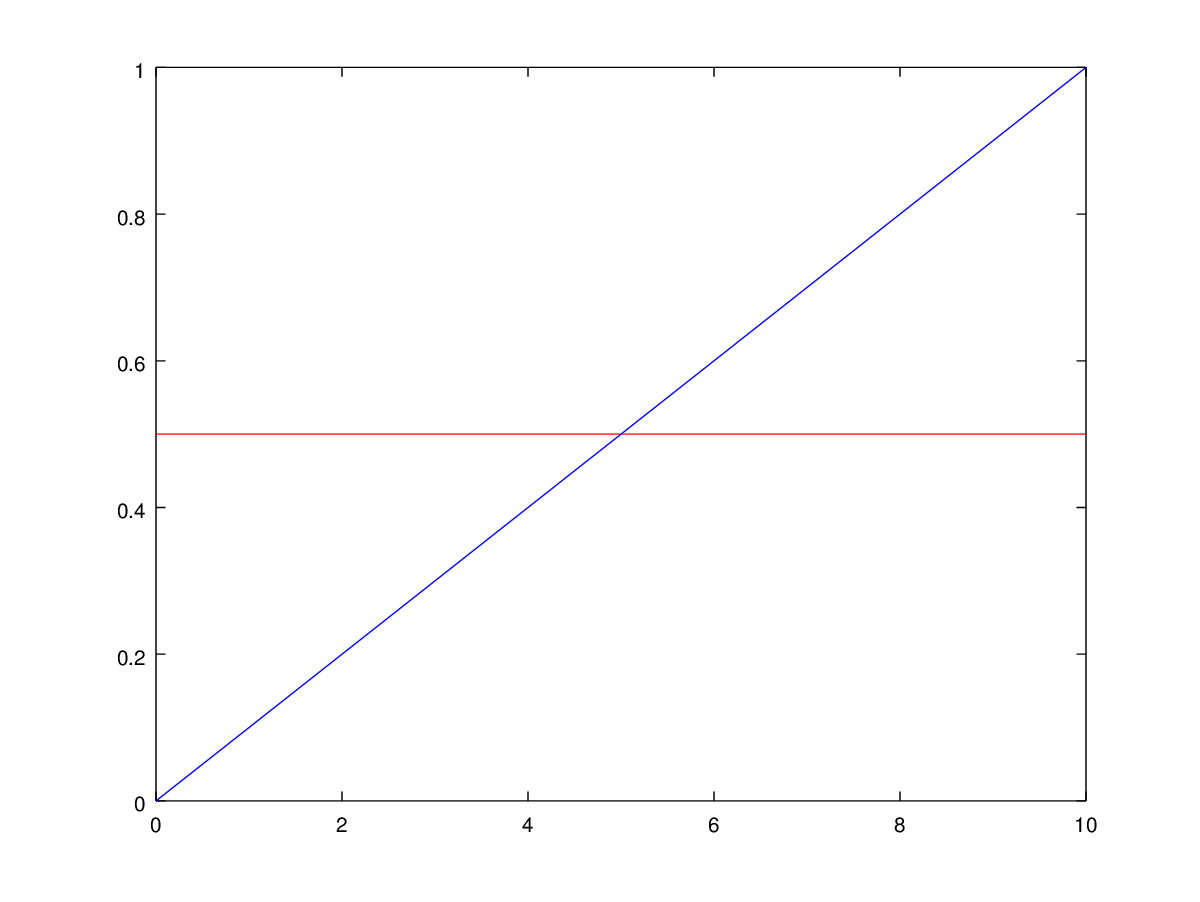
\includegraphics{expectation.png}\label{fig:expectation}
	}
\end{figure}
Clearly, for swipe gesture navigation, it is reasonable to assume that the
time required increases proportionally with the distance as the number of
swipes increases proportionally as well.  It is also reasonable to assume
constant time consumption for menu navigation as the page selection process
should be independent of $d$. However, this might not hold true when $d$ is so
large that the user is required to scroll within the menu in order to select
the desired page. In Figure~\ref{fig:expectation}, we presume the intercept
point between the lines to exist. The location, however, is part of our
research.  The user satisfaction is likely to be a monotonically decreasing
function in $d$. However, the shape of the function is unknown and will be
subject to our research as well.
Since we assume a linear function, we choose $d = 5, 10, 15, 20, 25$ as concrete
values for $d$.

The results of our research will give important insight into the usability of
different navigation methods, potentially leading to guidelines for the design
of future e-learning apps.


%%%%%%%%%%%%%%%%%%%%%%%%%%%%%%%%%%%%
For all our analyses, we used the scipy.stats package for Python.

Before we report the results for the data that are directly linked to our hypotheses formulated in Chapter 1, we look into
the results of the questionnaires that are designed to check the validity of our study's design. Task question (1) 
\todo{Put evaluation of task question (1) and final questions 1 - 3 here}.

Our main focus in this research is on comparing the two navigation methods when the distance is equal.
The results for all independent variables as introduced in Chapter \ref{chap:measurements} are shown in Table \ref{fig:burger-vs-swipe}. Recall that the
satisfaction is quantified through task question (2). For additional results please see the Appendix. 
In order to test for significant differences in any of the independent variables, we first apply \todo{test for
normality} to test for normality and apply Welch's t-test (marked with *) if we \todo{can or cannot reject something, depending on what test is used.} for both groups.
In the case of a t-test, we report the following data in this order: t value, significance level p and effect size \todo{Again, which measure if there are multiple
options}. The degrees of freedom is \ldots in all cases where a t-test is applied. \todo{verify: is it always the same?}.
In the case where the test for normality fails, we apply a Mann-Whitney-U test (marked with ~), in which case z value, significance level p, and effect size are provided.
\begin{table}[!h]
\centering
\caption{Comparing burger and swipe for same d}
\label{fig:burger-vs-swipe}
\resizebox{\columnwidth}{!}{
\begin{tabular}{@{}c|c|c|c@{}}
\toprule
d & effectiveness & efficiency & satisfaction   \\
\midrule 2 & ~ z, p, d & * t, p, d &         \\
\midrule 5 & * t, p, d & ~ z, p, d &         \\
\midrule 8 & & &         \\
\midrule 11 & & &         \\
\midrule 14 & & &         \\
\end{tabular}}
\end{table}

\subsection{Effectiveness}
Overall, \todo{how much?} \% of the tasks were solved optimally with burger menu and \todo{how much?} \% were solved optimally with swipe gestures. For burger menu navigation, 
Table \ref{fig:descriptive-effectiveness} shows that the error rates were slightly lower for task 1 and task 5 than for the others. However, the differences
are not significant (see Appendix). For the swipe navigation, the error rate of task 1 is significantly lower than the error rates of all the other
tasks (Table \todo{make table where swipe stuff is compared}). These are the only significances when comparing swipe among different distances. When
comparing both navigation methods applied to the same distances, significantly less errors are produced with burger menu on task 3, 4, and 5, but not on tasks 1 and 2.
\begin{table}[!h]
\centering
\caption{Mean (standard deviation) of effectiveness}
\label{fig:descriptive-effectiveness}
\resizebox{\columnwidth}{!}{
\begin{tabular}{|c|c|c|c|c|c|}
\toprule
navigation & 2 & 5 & 8 & 11 & 14  \\
\midrule burger & $\mu (\sigma)$ & $\mu (\sigma)$ & $\mu (\sigma)$ & $\mu (\sigma)$ & $\mu (\sigma)$ \\
\midrule swipe & $\mu (\sigma)$ & $\mu (\sigma)$ & $\mu (\sigma)$ & $\mu (\sigma)$ & $\mu (\sigma)$  \\
\end{tabular}}
\end{table}
\subsection{Efficiency}
Averaged over all tasks, the efficiency of burger (\todo{value, SD}) is slightly higher than the efficiency of swipe navigation (\todo{value, SD}). When looking at the
development of the means depending on the tasks is shown in Table \ref{fig:descriptive-efficiency}. \todo{Any tendency? Significances?}. When comparing the navigation methods with each other,
we can observe that \todo{what} is significantly better than \todo{what} in tasks \todo{which ones}, whereas the relation is flipped in tasks \todo{which ones}. For tasks \todo{which ones},
no significances can be found.
\begin{table}[!h]
\centering
\caption{Mean (standard deviation) of efficiency}
\label{fig:descriptive-efficiency}
\resizebox{\columnwidth}{!}{
\begin{tabular}{|c|c|c|c|c|c|}
\toprule
navigation & 2 & 5 & 8 & 11 & 14  \\
\midrule burger & $\mu (\sigma)$ & $\mu (\sigma)$ & $\mu (\sigma)$ & $\mu (\sigma)$ & $\mu (\sigma)$ \\
\midrule swipe & $\mu (\sigma)$ & $\mu (\sigma)$ & $\mu (\sigma)$ & $\mu (\sigma)$ & $\mu (\sigma)$  \\
\end{tabular}}
\end{table}
\subsection{Satisfaction}
The average rating of task question 2, our main measurement for the user's satisfaction with the navigation method, is \todo{avg rating} for the burger menu group and \todo{avg rating}
for the swipe gesture group. This \todo{matches or doesn't match} the results from final question (4), where the burger menu and swipe gestures yield a rating of \todo{value} and \todo{value} 
on average, respectively. See Table \ref{fig:descriptive-satisfaction} for the statistics of individual tasks. It can be seen that \todo{what can be seen}.
\begin{table}[!h]
\centering
\caption{Mean (standard deviation) of satisfaction}
\label{fig:descriptive-satisfaction}
\resizebox{\columnwidth}{!}{
\begin{tabular}{|c|c|c|c|c|c|}
\toprule
navigation & 2 & 5 & 8 & 11 & 14  \\
\midrule burger & $\mu (\sigma)$ & $\mu (\sigma)$ & $\mu (\sigma)$ & $\mu (\sigma)$ & $\mu (\sigma)$ \\
\midrule swipe & $\mu (\sigma)$ & $\mu (\sigma)$ & $\mu (\sigma)$ & $\mu (\sigma)$ & $\mu (\sigma)$  \\
\end{tabular}}
\end{table}
\section{Discussion}
\subsection{Effectiveness}
Maybe effectiveness doesn't have a large meaning the way we defined it? Making an error may be less of an issue because it takes away less time.

Explain relatively large success rates for task 1 and 5 (burger).
Results may indicate that swipe is preferable for small distances, because error rate is rather low and making an error may potentially be not as bad
with swipe. Recall no significant differences between burger and swipe. 
\subsection{Efficiency}
\subsection{Satisfaction}
Task question 1 should maybe have been more specific? Final questions (3) and (4) too similar, hard to distinguish (that was a participant's comment)?
\section{Related Work}
\section{Conclusions}
Conclusions
%\end{document}  % This is where a 'short' article might terminate

%ACKNOWLEDGMENTS are optional
\section{Acknowledgments}

%
% The following two commands are all you need in the
% initial runs of your .tex file to
% produce the bibliography for the citations in your paper.
\bibliographystyle{abbrv}
\bibliography{hci}  % sigproc.bib is the name of the Bibliography in this case
% You must have a proper ".bib" file
%  and remember to run:
% latex bibtex latex latex
% to resolve all references
%
% ACM needs 'a single self-contained file'!
%
%APPENDICES are optional
%\balancecolumns
\newpage
\onecolumn
\appendix%Appendix A
\todo{We use a t-test for DEPENDENT samples}
\section{Some Appendices}
tables and stuff

\begin{table}[!h]
	\centering
	\caption{Course distribution}
	\label{tab:course}
	\begin{tabular}{@{}p{14cm}|c}
		\toprule
		\textbf{Course} & \textbf{Count} \\
		\midrule Wirtschaftsinformatik & 6 \\
		\midrule Agrarwissenschaften & 5 \\
		\midrule Mathematik & 4 \\
		\midrule Psychologie & 4 \\
		\midrule Volkswirtschaftslehre & 3 \\
		\midrule Ernährungs- und Verbraucherökonomie & 2 \\
		\midrule Finanzmathematik & 2 \\
		\midrule Wirtschaftsingenieur & 2 \\
		\midrule Agribusiness & 1 \\
		\midrule Betriebswirtschaftslehre & 1 \\
		\midrule Biochemie & 1 \\
		\midrule Biologie & 1 \\
		\midrule Informatik & 1 \\
		
		\midrule Mathematik / Chemie & 1 \\
		\midrule Mathematik / Deutsch / Psychologie & 1 \\
		\midrule Mathematik / Geologie & 1 \\
		\midrule Mathematik / Geschichte & 1 \\
		\midrule Mathematik / Informatik & 1 \\
		\midrule Mathematik / Philosophie & 1 \\
		\midrule Mathematik / Physik & 1 \\
		\midrule Mathematik / Spanisch & 1 \\
		\midrule Mathematik / Sport & 1 \\
		
		\midrule Medizin & 1 \\
		\midrule Musikwissenschaft / Philosophie & 1 \\
		\midrule Physik & 1 \\
		\midrule Politikwissenschaft / Ur- und Frühgeschichte & 1 \\
		\midrule Rechtswissenschaften & 1 \\
		\midrule Soziologie / Pädagogik & 1 \\
		\midrule Wirtschaftswissenschaften Profil: Handelslehrer & 1 \\
		\midrule N/A (1-Fa-Ma) & 1 \\
	\end{tabular}
\end{table}

\end{document}
